%! Author = Len Washington III
%! Date = 2/25/24

% Preamble
\documentclass[title={Chapter 7}]{fdsn201notes}

% Packages

% Document
\begin{document}

%<*Chapter7>
\maketitle{7}{Nutrients Essential to Fluid and Electrolyte Balance}%

\section{Fluids}\label{sec:fluids}
\begin{itemize}
	\item Substances composed of freely moving molecules
	\item Have the ability to conform to the shape of the container that holds them
	\item There are different types of fluids in our bodies
	\begin{itemize}
		\item $\frac{2}{3}$ of the body's fluid is \emph{intracellular fluid}
		\item The remaining $\frac{1}{3}$ is \emph{extracellular fluid}
	\end{itemize}
\end{itemize}

\begin{figure}[H]
	\centering
	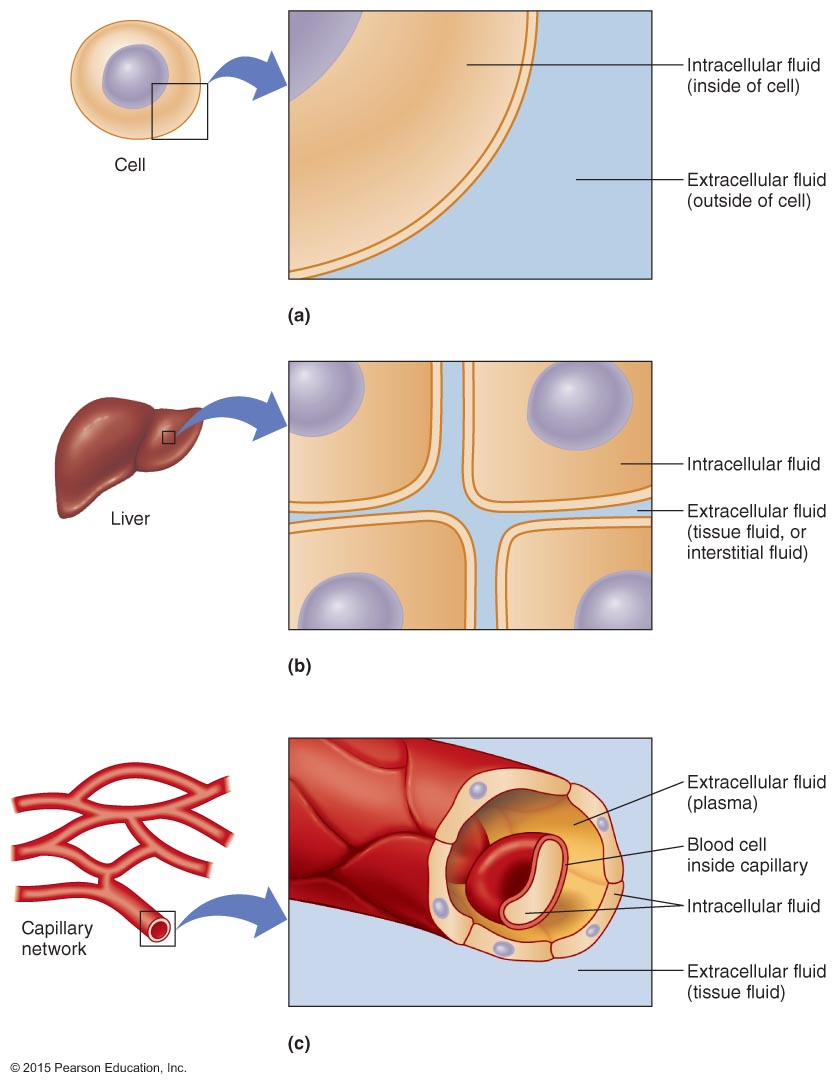
\includegraphics[width=\textwidth]{7_components_of_body_fluid}
	\caption{Components of Body Fluid}
	\label{fig:components_of_body_fluid}
\end{figure}

\begin{itemize}
	\item Extracellular fluids include
	\begin{itemize}
		\item \definition{Tissue fluid}{found between the cells within tissues and organs of the body}
		\item \definition{Plasma}{the fluid portion of blood that carries the blood cells}
	\end{itemize}
	\item The body fluid composition of tissue varies by
	\begin{description}
		\item[Tissue type] lean tissues have higher fluid content than fat tissues
		\item[Gender] males have more lean tissue and therefore more body fluid
		\item[Age] lean tissue is lost with age, and body fluid is lost with it
	\end{description}
\end{itemize}

\section{Electrolytes}\label{sec:electrolytes}
\begin{itemize}
	\item In intracellular fluid, $\mbox{K}^{+}$ and $\mbox{HPO}_{4}^{2-}$ are the predominant electrolytes
	\item In extracellular fluid, $\mbox{Na}^{+}$ and $\mbox{Cl}^{-}$ predominate
	\item There is a slight electrical charge difference on either side of the cell membrane
\end{itemize}

\section{Functions of Fluids}\label{sec:functions-of-fluids}
\begin{itemize}
	\item Fluids dissolve and transport substances
	\begin{itemize}
		\item Water is an excellent \emph{solvent} because it can dissolve many different substances
		\item The dissolved materials, or \emph{solutes}, include ions, carbohydrates, amino acids, vitamins, and minerals
	\end{itemize}
	\item Fluids account for blood volume
	\begin{itemize}
		\item \definition{Blood volume}{the amount of fluid in the blood}
		\item Increased blood volume can cause blood pressure to rise (hypertension)
		\item Decreased blood volume can cause low blood pressure
	\end{itemize}
	\item Fluids help maintain body temperature
	\begin{itemize}
		\item Because water has a high heat capacity, the temperature of our body fluids remain quite stable
		\item Sweating releases heat as the evaporation of water from the skin cools the skin and blood
	\end{itemize}
\end{itemize}

\begin{figure}[H]
	\centering
	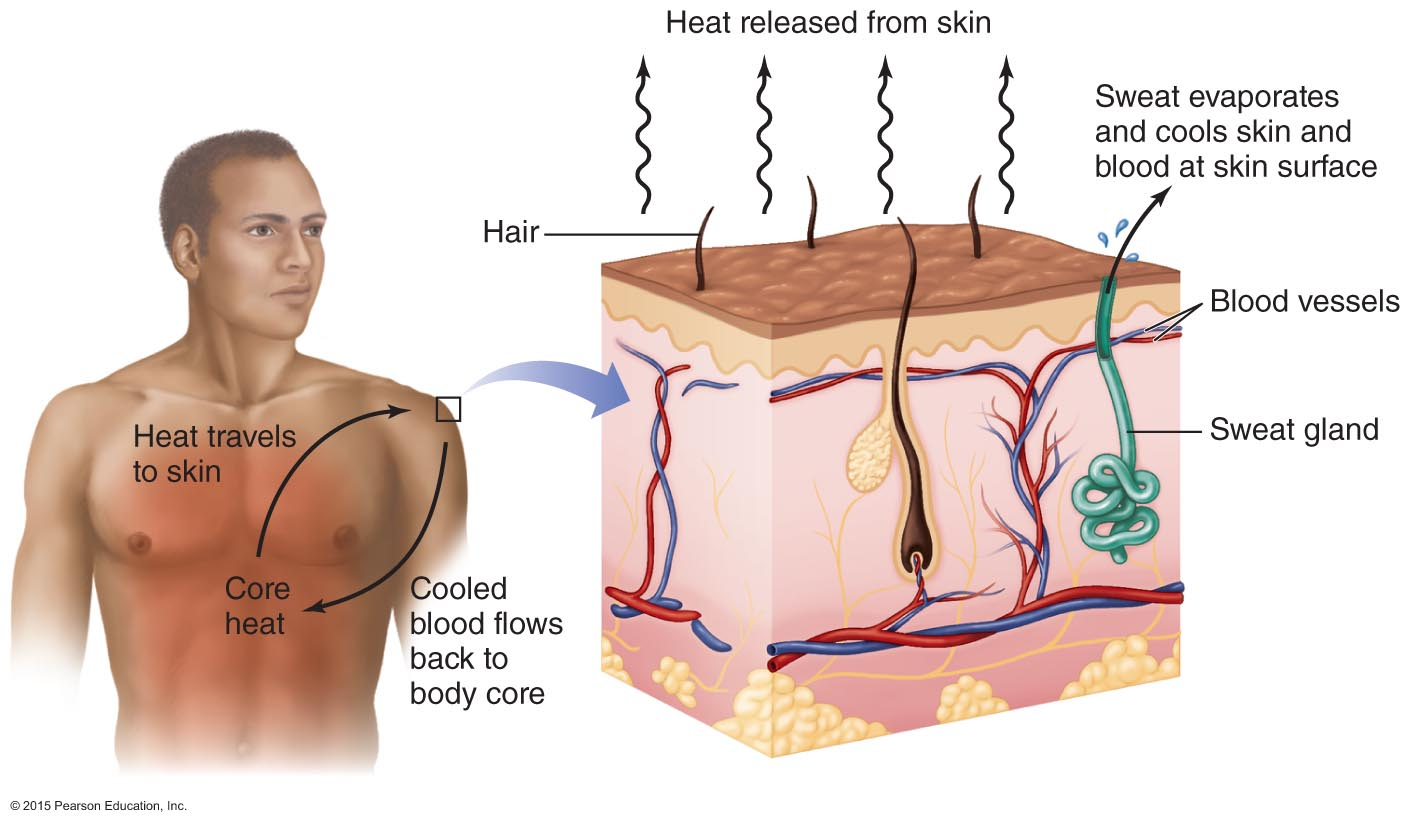
\includegraphics[width=\textwidth]{7_fluids_help_maintain_body_temperature}
	\caption{Fluids Help Maintain Body Temperature}
	\label{fig:7_fluids_help_maintain_body_temperature}
\end{figure}

\begin{itemize}
	\item Fluids protect and lubricate our tissues
	\begin{itemize}
		\item Cerebrospinal fluid protects the brain and spinal column
		\item Amniotic fluid protects the fetus
		\item Synovial fluid is a lubricant around joints
		\item Digestive secretions allow for easy passage
		\item Pleural fluid covering the lungs allows friction-free expansion and retraction
	\end{itemize}
\end{itemize}

\section{Functions of Electrolytes}\label{sec:functions-of-electrolytes}
\begin{itemize}
	\item Electrolytes help regulate fluid balance
	\begin{itemize}
		\item Water follows the movement of electrolytes, moving by osmosis to areas where the concentration of electrolytes is high
		\item This allows for the controlled movement of fluids into and out of cells
	\end{itemize}
\end{itemize}

\begin{figure}[H]
	\centering
	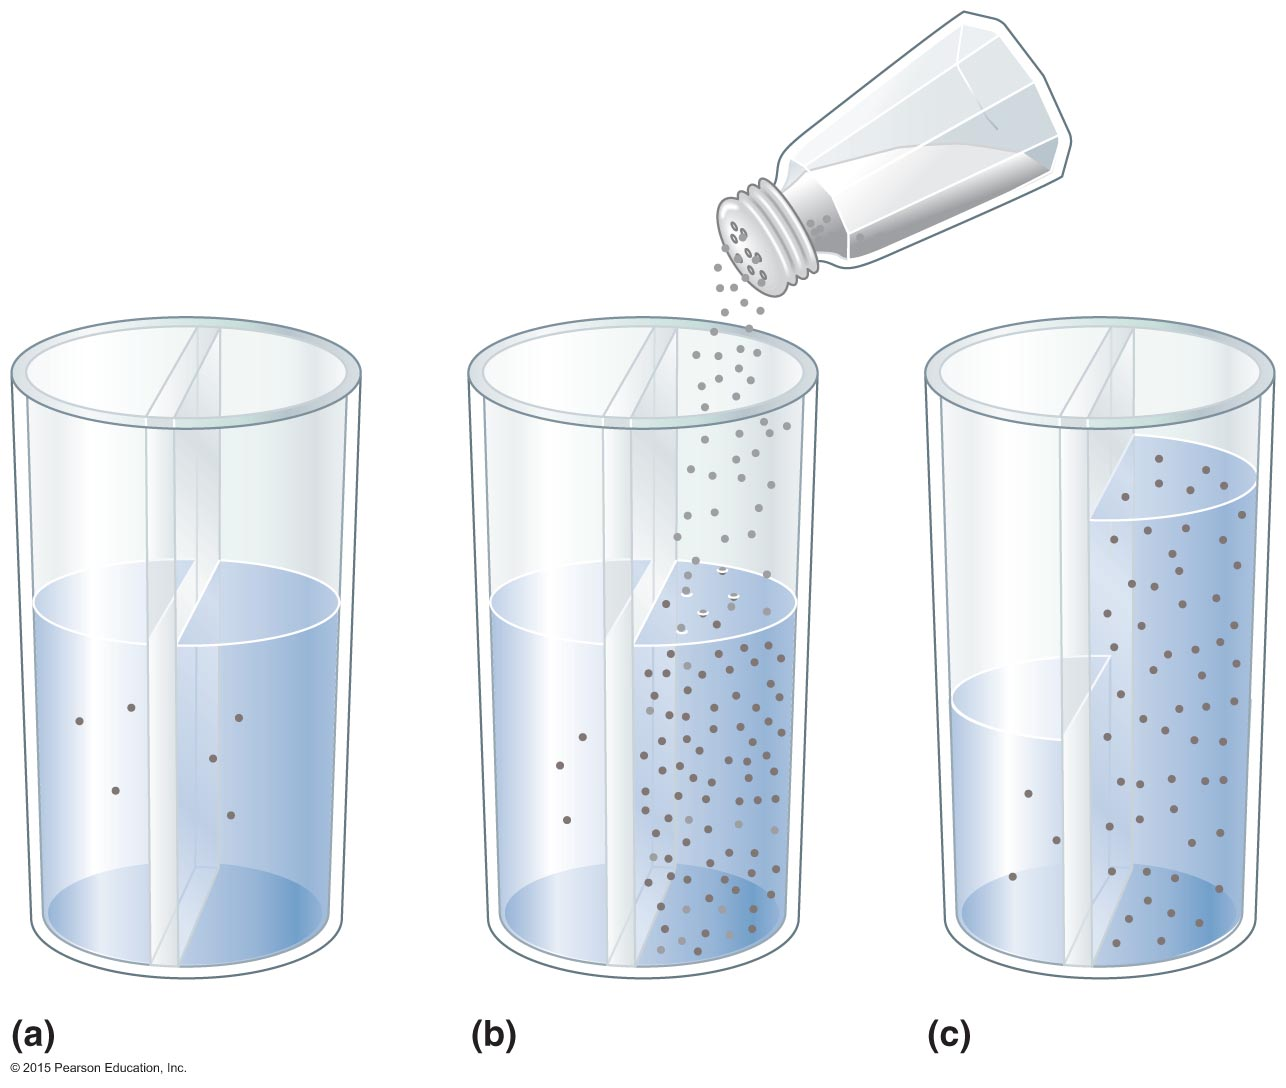
\includegraphics[width=\textwidth]{7_osmosis}
	\caption{Osmosis}
	\label{fig:7_osmosis}
\end{figure}

\begin{figure}[H]
	\centering
	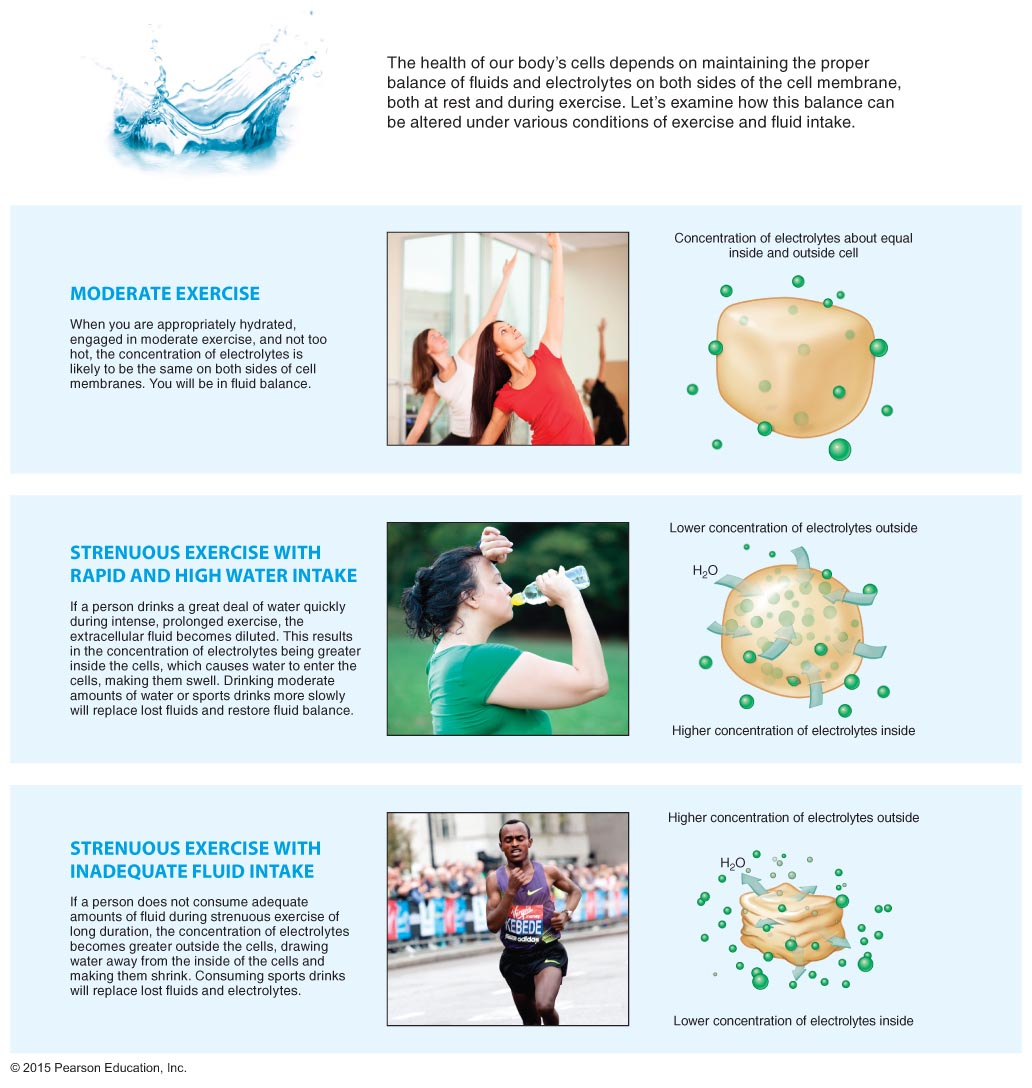
\includegraphics[width=\textwidth]{7_fluid_and_electrolyte_balance}
	\caption{Fluid and Electrolyte Balance}
	\label{fig:fluid_and_electrolyte_balance}
\end{figure}

\begin{itemize}
	\item Electrolytes enable our nerves to respond to stimuli
	\begin{itemize}
		\item Movement of sodium ($\mbox{Na}^{+}$) and potassium $(\mbox{K}^{+})$ across the membranes of nerve cells changes the electrical charge across the membrane
		\item This change in electrical charge carries the nerve impulse along the nerve cell
	\end{itemize}
\end{itemize}

\begin{figure}[H]
	\centering
	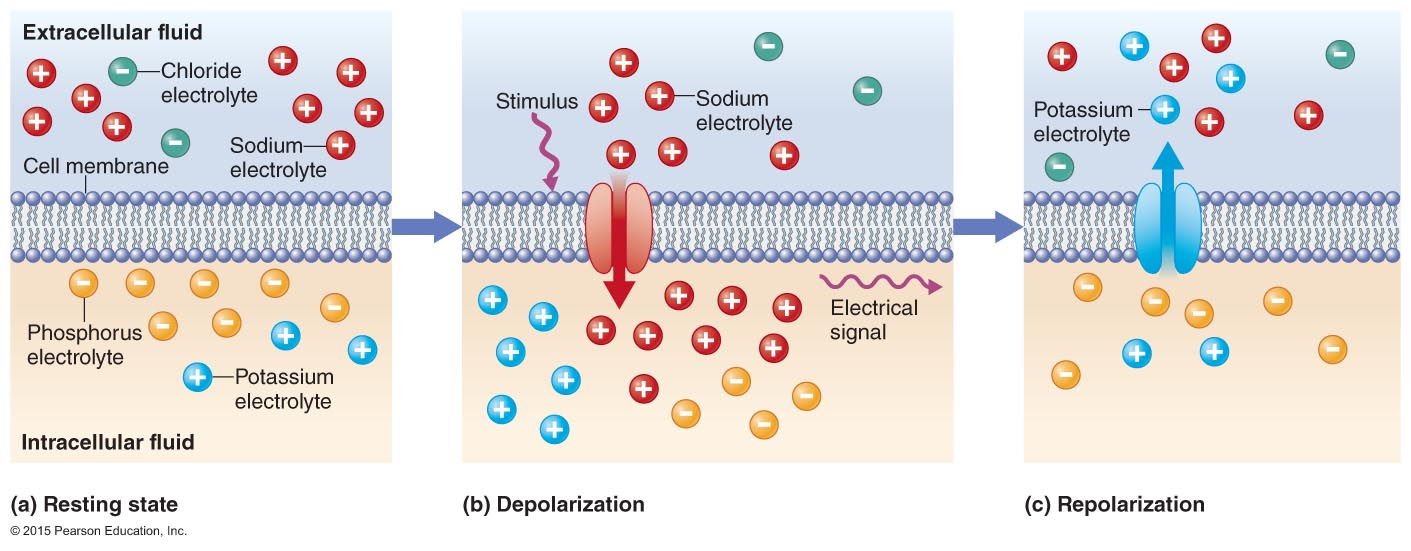
\includegraphics[width=\textwidth]{7_role_of_electrolytes_in_nerve_function}
	\caption{Role of Electrolytes in Nerve Function}
	\label{fig:7_role_of_electrolytes_in_nerve_function}
\end{figure}

\begin{itemize}
	\item Electrolytes signal our muscles to contract
	\begin{itemize}
		\item The movement of calcium ($\mbox{Ca}^{2+}$) into a muscle cell stimulates the muscle to contract
		\item The ($\mbox{Ca}^{2+}$) is pumped back out of the cell after the muscle contraction
	\end{itemize}
\end{itemize}

\section{Maintaining Fluid Balance}\label{sec:maintaining-fluid-balance}
\begin{itemize}
	\item Fluid balance is maintained by different mechanisms prompting us to drink and retain fluid
	\item The \emph{thirst mechanism} occurs from a cluster of nerve cells (in the hypothalamus) that stimulate our desire to drink
	\item However, the thirst mechanism is not always sufficient; the amount of fluids people drink may not be enough to achieve fluid balance
	\item Water lost from the body must be replaced
	\item Water is lost through urine, sweat, evaporation, exhalation, and feces
	\item Water is gained through beverages, food, and metabolic reactions
	\begin{itemize}
		\item \emph{Metabolic water} contributes about 10--14\% of the water the body needs
	\end{itemize}
\end{itemize}

\begin{figure}[H]
	\centering
	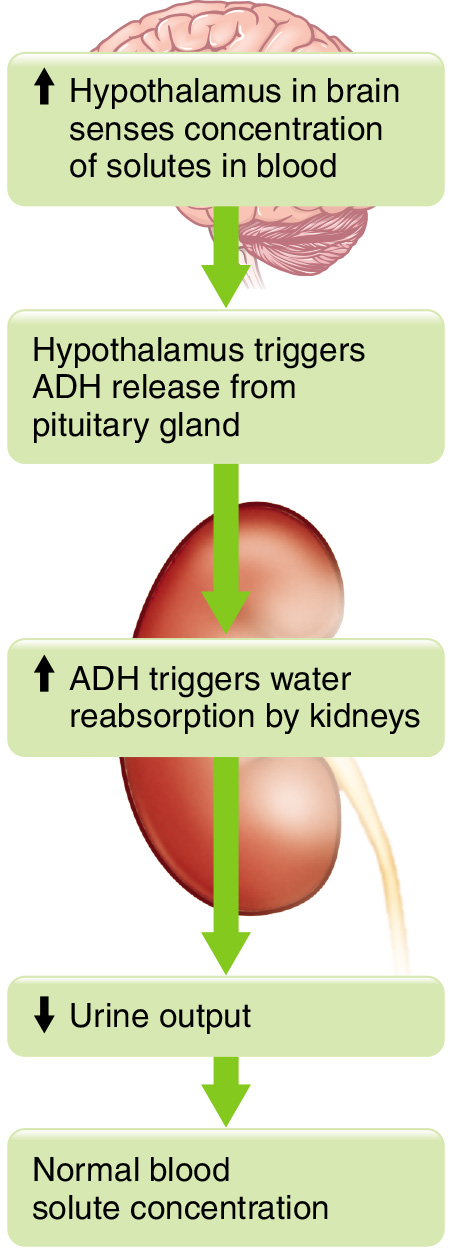
\includegraphics[height=0.5\paperheight]{7_fluid_balance}
	\caption{Fluid Balance}
	\label{fig:fluid_balance}
\end{figure}

\begin{figure}[H]
	\centering
	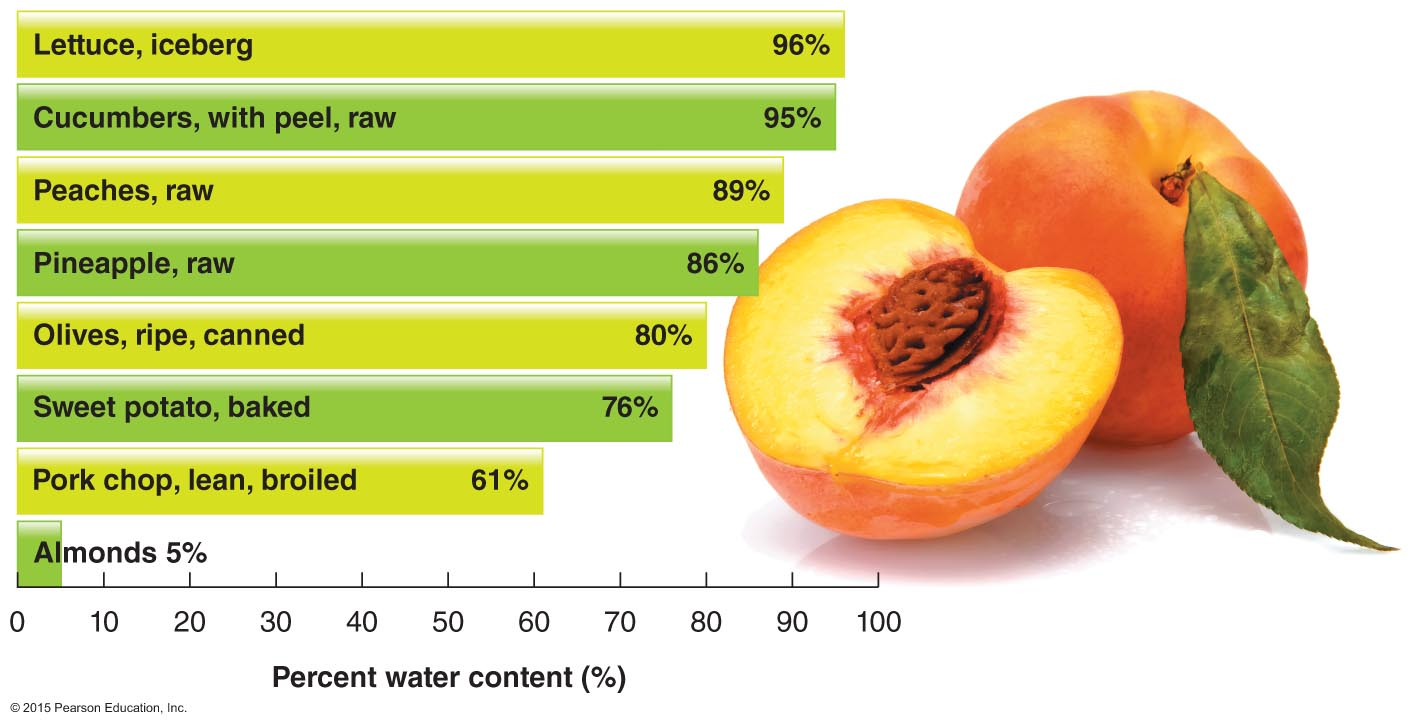
\includegraphics[width=\textwidth]{7_water_content_of_various_foods}
	\caption{Water Content of Various Foods}
	\label{fig:water_content_of_various_foods}
\end{figure}

\begin{itemize}
	\item Loss of water
	\begin{description}
		\item[Sensible water loss] occurs through urine and sweat
		\begin{itemize}
			\item Most water is lost through urine
			\item The kidneys control how much water is reabsorbed; excess water is processed by the kidneys and excretes as urine
		\end{itemize}
		\item[Insensible water loss] occurs through evaporation from the skin or exhalation from the lungs, as well as through feces
		\item[Diuretics] increase fluid loss via the urine
	\end{description}
\end{itemize}

\section{Water}\label{sec:water}
\begin{itemize}
	\item Functions of water
	\begin{itemize}
		\item Essential for life
		\item Required for fluid and electrolyte balance and many metabolic reactions
	\end{itemize}
	\item Recommended intake
	\begin{itemize}
		\item Varies with environment and activity level
	\end{itemize}
\end{itemize}

\begin{figure}[H]
	\centering
	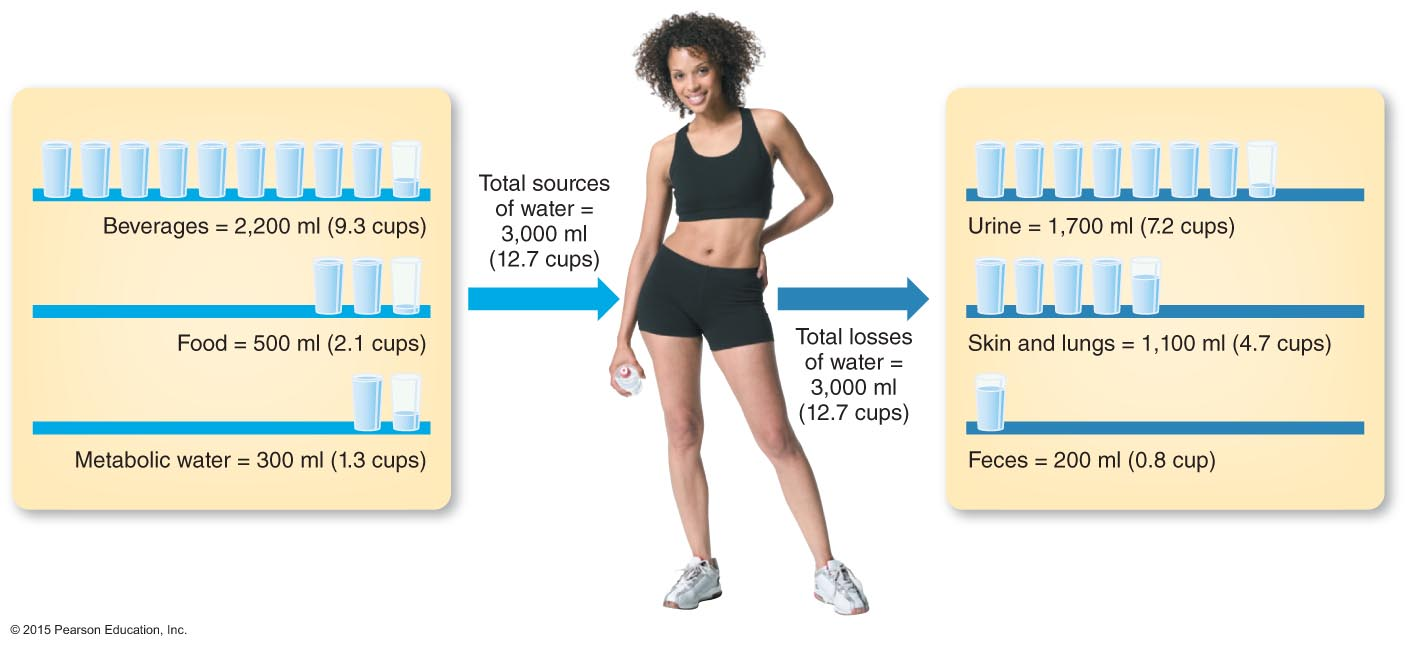
\includegraphics[width=\textwidth]{7_woman_expenditure}
	\caption{For a Woman Expending 2,500 kcal/day}
	\label{fig:woman_expenditure}
\end{figure}

\begin{itemize}
	\item Surface water comes from lakes, rivers, and reservoirs
	\item Groundwater comes from underground rock formations called aquifers
	\item ``Hard water'' is relatively high in calcium
	\item The U.S.\ Environmental Protection Agency (EPA) sets and monitors standards for public water systems and is responsible for regulation of bottled water
	\item What is you drink too much water?
	\begin{itemize}
		\item Becoming overhydrated is rare
		\item Can resulted in a dilution of sodium (hyponatremia)
	\end{itemize}
	\item What is you don't drink enough water?
	\begin{itemize}
		\item Dehydration
		\item Infants and the elderly are especially vulnerable
	\end{itemize}
\end{itemize}

\section{Commercial Beverages}\label{sec:commercial-beverages}
\begin{itemize}
	\item Low-fat and skim milk provide protein, calcium, phosphorus, vitamin D, and, usually, vitamin A
	\item Moderate consumption of beverages with caffeine is safe and potentially healthful
	\item Most soft drinks, juice drinks, flavored waters, and bottled tea and coffee drinks are loaded with added sugars
	\item ``Designer waters'' with added nutrients and/or herbs can add more than 300 Calories to the day's intake and rarely contribute to better health
	\item Many energy drinks, typically consumed quickly, contain a high amount of caffeine, which can cause a dramatic rise in blood pressure and heart rate
	\begin{itemize}
		\item The can also contain a significant amount of added sugar
	\end{itemize}
\end{itemize}

\begin{table}[H]
	\centering
	\begin{adjustbox}{max width=0.95\paperwidth,center}
		\begin{threeparttable}
			\caption{Overview of Minearls Involved in Hydration and Neuromuscular Function}
			\label{tab:minerals_in_hydration}
			\rowcolors{2}{rowmedgreen}{rowlightgreen}
			\begin{tabular}{p{0.125\paperwidth} p{0.7\paperwidth}}
				\rowcolor{rowdarkgreen}\textbf{Nutrient} & \textbf{Recommended Intake}\\
				Sodium & AI for 19 to 50 years of age: 1.5 g/day\\
				Potassium & AI for 19 years of age and older: 4.7 g/day\\
				Chloride & AI for 19 to 50 years of age: 2.3/day\\
				Phosphorus & RDA for 19 years of age and older: 700 mg/day\\
				\rowcolor{rowdarkgreen} & \\
			\end{tabular}
			\begin{tablenotes}
				\small
				\item To see the full profile of all micronutrients, turn to the \textbf{In Depth} essay following Chapter 6, Vitamins and Minerals: Micronutrients with Macro Powers (pages 211--221).
			\end{tablenotes}
		\end{threeparttable}
	\end{adjustbox}
\end{table}

\section{Sodium}\label{sec:sodium}
\begin{itemize}
	\item Functions of sodium
	\begin{itemize}
		\item Fluid and electrolyte balance
		\item Associated with blood pressure and pH balance in the body
		\item Required for nerve impulse transmission
		\item Assists in the transport of certain nutrients (e.g., glucose) into body cells
	\end{itemize}
	\item Recommended intake
	\begin{itemize}
		\item 1.5 g/day is required
		\item No more than 2.3 g/day is recommended
	\end{itemize}
	\item Sources of sodium
	\begin{itemize}
		\item Processed foods and restaurant foods are generally high in sodium
	\end{itemize}
\end{itemize}

\begin{table}[H]
	\centering
	\begin{adjustbox}{max width=0.95\paperwidth,center}
		\begin{threeparttable}
			\caption{High-Sodium Foods and Lower-Sodium Alternatives}
			\label{tab:sodium-alternatives}
			\rowcolors{2}{rowmedgreen}{rowlightgreen}
			\begin{tabular}{*{2}{p{0.375\paperwidth} C{0.125\paperwidth} }}
				\rowcolor{rowdarkgreen}\textbf{High-Sodium Food} & \textbf{Sodium (mg)} & \textbf{Lower-Sodium Food} & \textbf{Sodium (mg)}\\
				Dill pickle (1 large, 4 in.) & 1,731 & Low-sodium dill pickle (1 large, 4 in) & 23\\
				Ham, cured, roasted (3 oz) & 1,023 & Pork, loin roast (3 oz) & 54\\
				Turkey pastrami (3 oz) & 915 & Roasted turkey, cooked (3 oz) & 54\\
				Tomato juice, regular (1 cup) & 877 & Tomato juice, lower sodium (1 cup) & 24\\
				Macaroni and cheese (1 cup) & 800 & Spanish rice (1 cup) & 5\\
				Ramen noodle soup (chicken flavor) (1 package [85 g]) & 1,960 & Ramen noodle soup made with sodium-free chicken bouillon (1 cup) & 0\\
				Teriyaki chicken (1 cup) & 3,210 & Stir-fried pork/rice/vegetables (1 cup) & 575\\
				Tomato sauce, canned ($\frac{1}{2}$ cup) & 741 & Fresh tomato (1 medium) & 11\\
				Creamed corn, canned (1 cup) & 730 & Cooked corn, fresh (1 cup) & 28\\
				Tomato soup, canned (1 cup) & 695 & Lower-sodium tomato soup, canned (1 cup) & 480\\
				Potato chips, salted (1 oz) & 168 & Baked potato, unsalted (1 medium) & 14\\
				Saltine crackers (4 crackers) & 156 & Saltine crackers, unsalted (4 crackers) & 100\\
				\rowcolor{rowdarkgreen} & & & \\
			\end{tabular}
			\begin{tablenotes}
				\small
				\item \textit{Data from: } U.S\@. Department of Agriculture.
				2011. USDA Nutrient Database for Standard Reference, Release 24.
			\end{tablenotes}
		\end{threeparttable}
	\end{adjustbox}
\end{table}

\begin{itemize}
	\item What is you consume too much sodium?
	\begin{itemize}
		\item \definition{Hypernatremia}{abnormally high blood sodium concentration}
		\item Can occur in patients with congestive heart failure or kidney disease
		\item Results in high blood volume, edema, and high blood pressure
	\end{itemize}
	\item What is you don't consume enough sodium?
	\begin{itemize}
		\item \definition{Hyponatremia}{an abnormally low blood sodium level}
		\item Can result from prolonged vomiting, diarrhea, or sweating
		\item Has been seen in marathon athletes who consume too much water and fail to replace sodium
	\end{itemize}
\end{itemize}

\section{Potassium}\label{sec:potassium}
\begin{itemize}
	\item Functions of potassium
	\begin{itemize}
		\item Fluid and electrolyte balance
		\item Very important in muscle contractions and transmission of nerve impulses
		\item High potassium intake helps to maintain a lower blood pressure
	\end{itemize}
	\item Recommended intake
	\begin{itemize}
		\item 4.7 g/day
	\end{itemize}
	\item Sources of potassium
	\begin{itemize}
		\item Processed foods are usually low in potassium
		\item Fresh fruit and vegetables and whole grains are good sources of potassium
	\end{itemize}
\end{itemize}

\begin{figure}[H]
	\centering
	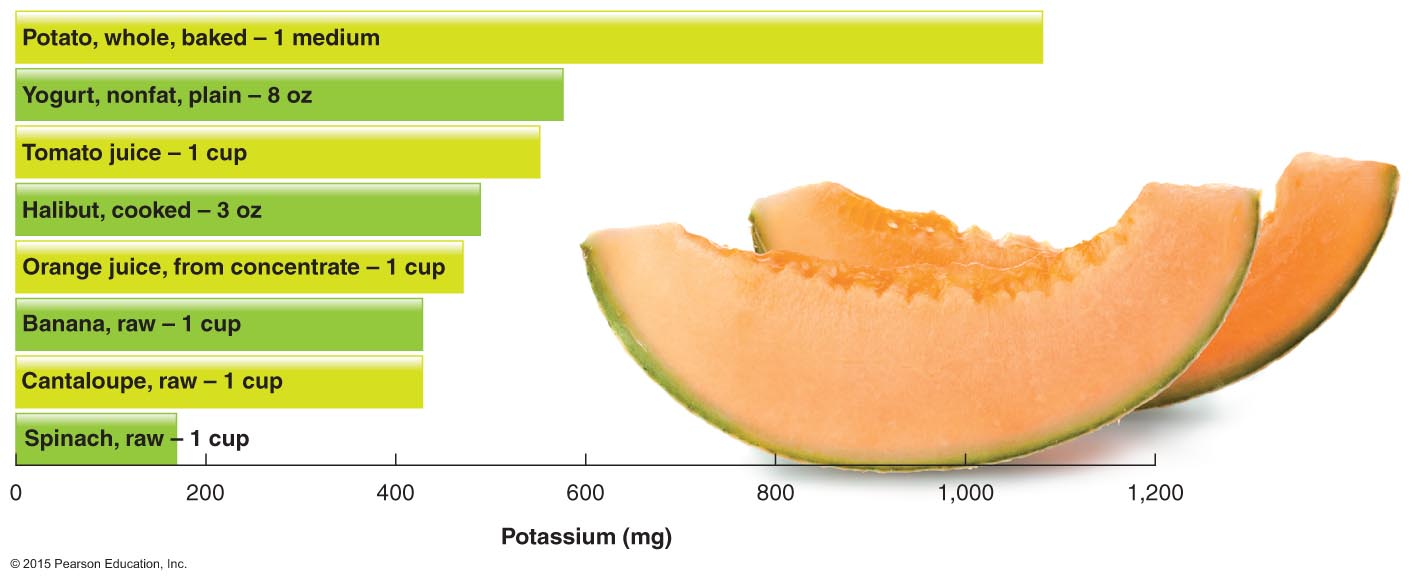
\includegraphics[width=\textwidth]{7_common_food_sources_of_potassium}
	\caption{Common Food Sources of Potassium}
	\label{fig:common_food_sources_of_potassium}
\end{figure}

\begin{itemize}
	\item What if you consume too much potassium?
	\begin{itemize}
		\item \definition{Hyperkalemia}{a high blood potassium level}
		\item Can occur in patients with kidney disease
		\item Can alter normal heart rhythm, resulting in a heart attach
	\end{itemize}
	\item What if you don't consume enough potassium?
	\begin{itemize}
		\item \definition{Hypokalemia}{a low blood potassium level}
		\item Can be seen in patients with kidney disease or diabetic acidosis
		\item Can occur when taking certain diuretic medications
	\end{itemize}
\end{itemize}

\section{Chloride}\label{sec:chloride}
\begin{itemize}
	\item Functions of chloride
	\begin{itemize}
		\item Assists with maintaining fluid balance
		\item Assists the immune system
		\item Component of HCl in the stomach
	\end{itemize}
	\item Recommended intake
	\begin{itemize}
		\item Minimum recommendation is 2.3 g/day
	\end{itemize}
	\item What if you consume too much chloride?
	\begin{itemize}
		\item May lead to hypertension in salt-sensitive patients
	\end{itemize}
	\item What if you don't consume enough chloride?
	\begin{itemize}
		\item This is rare but can occur in people with eating disorders
	\end{itemize}
\end{itemize}

\section{Phosphorus}\label{sec:phosphorus}
\begin{itemize}
	\item Functions of phosphorus
	\begin{itemize}
		\item The major intracellular negatively charged electrolyte
		\item Required for fluid balance
		\item Critical role in bone formation (85\% of body's phosphorus is found in bone)
		\item Regulated biochemical pathways by activating or deactivating enzymes
		\item Found in ATP, DNA, RNA
	\end{itemize}
	\item Recommended intake
	\begin{itemize}
		\item Recommended Dietary Allowance (RDA) for phosphorus is 700 mg/day
	\end{itemize}
	\item Sources of phosphorus
	\begin{itemize}
		\item Widespread in many foods
		\item Found in high amounts in foods that contain protein (e.g., meat, milk, eggs)
	\end{itemize}
\end{itemize}

\begin{figure}[H]
	\centering
	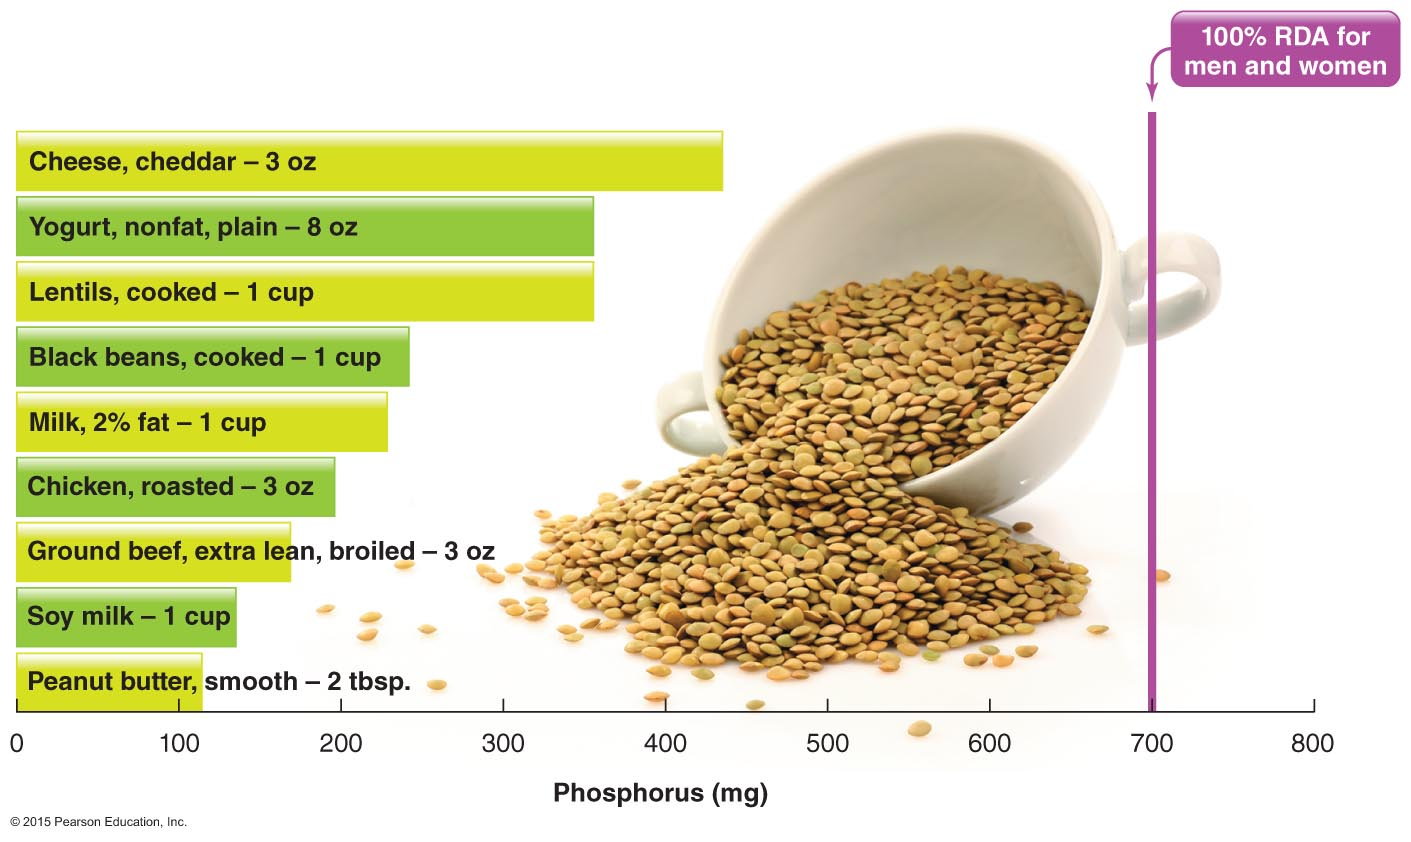
\includegraphics[width=\textwidth]{7_common_food_sources_of_phosphorus}
	\caption{Common Food Sources of Phosphorus}
	\label{fig:common_food_sources_of_phosphorus}
\end{figure}

\begin{itemize}
	\item What if you consume too much phosphorus?
	\begin{itemize}
		\item High blood levels of phosphorus can occur with kidney disease or when taking too much vitamin D supplements
		\item Causes muscles spams, and convulsions
	\end{itemize}
	\item What if you don't consume enough phosphorus?
	\begin{itemize}
		\item Deficiencies of phosphorus are rare
	\end{itemize}
\end{itemize}

\section{Fluid and Electrolyte Balance Disorders}\label{sec:fluid-and-electrolyte-balance-disorders}
\begin{itemize}
	\item Serious health problems that can occur when fluid excretion exceeds fluid intake include
	\begin{itemize}
		\item Dehydration
		\begin{itemize}
			\item Occurs when fluid excretion exceeds fluid intake
		\end{itemize}
		\item Heat illnesses
		\begin{itemize}
			\item Heat cramps
			\item Heat exhaustion
			\item Heat stroke
		\end{itemize}
	\end{itemize}
\end{itemize}

\section{Dehydration}\label{sec:dehydration}
\begin{itemize}
	\item Occurs when water loss exceeds water intake
	\begin{itemize}
		\item Commonly due to heavy exercise or high environmental temperatures
		\item Infants and the elderly are more at risk
	\end{itemize}
	\item Other common causes of dehydration include
	\begin{itemize}
		\item Diarrhea
		\item Vomiting
		\item Fever
		\item Burns, including sunburn
		\item Poorly controlled diabetes
		\item Abuse of diuretics or laxatives
	\end{itemize}
	\item Dehydration is classified in terms of percentage of weight loss that is exclusively due to the loss of fluids
\end{itemize}

\begin{table}[H]
	\centering
	\begin{adjustbox}{max width=0.95\paperwidth,center}
		\begin{threeparttable}
			\caption{Percentages of Body Fluid Loss Correlated with Weight Loss and Symptoms}
			\label{tab:fluid-loss-percentages}
			\rowcolors{2}{rowmedgreen}{rowlightgreen}
			\begin{tabular}{p{0.12\paperwidth} p{0.2\paperwidth}p{0.2\paperwidth}p{0.48\paperwidth}}
				\rowcolor{rowdarkgreen}\textbf{Body Water Loss (\%)} & \textbf{Weight Lost If You Weight 160 lb} & \textbf{Weight Lost If You Weight 130 lb} & \textbf{Symptoms}\\
				1--2 & 1.6--3.2 lb & 1.3--2.6 lb & Strong thirst, loss of appetite, feeling uncomfortable\\
				3--5 & 4.8--8.0 lb & 3.9--6.5 lb & Dry mouth, reduced urine output, greater difficulty working and concentrating, flushed skin, tingling extremities, impatience, sleepiness, nausea, emotional instability\\
				6--8 & 9.6--12.8 lb & 7.8--10.4 lb & Increased body temperature that doesn't decrease, increased heart rate and breathing rate, dizziness, difficulty breathing, slurred speech, mental confusion, muscle weakness, blue lips\\
				9--11 & 14.4--17.6 lb & 11.7--14.3 lb & Muscle spasms, delirium, swollen tongue, poor balance, and circulation, kidney failure, decreased blood volume and blood pressure\\
				\rowcolor{rowdarkgreen} & & & \\
			\end{tabular}
			\begin{tablenotes}
				\small
				\item \textit{Data from: Nutrition and Aerobic Exercise,} edited by D. K. Layman.
				\textcopyright 1986 American Chemical Society.
			\end{tablenotes}
		\end{threeparttable}
	\end{adjustbox}
\end{table}

\begin{figure}[H]
	\centering
	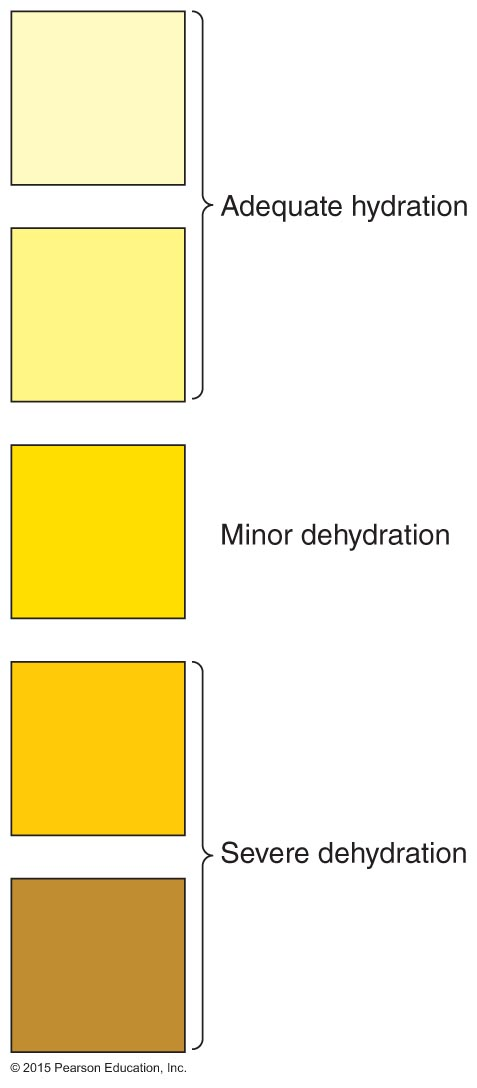
\includegraphics[height=0.5\paperheight]{7_using_urine_color_to_gauge_hydration}
	\caption{Using Urine Color to Gauge Hydration}
	\label{fig:using_urine_color_to_gauge_hydration}
\end{figure}

\section{Heat Illnesses}\label{sec:heat-illnesses}
\begin{itemize}
	\item Three common types of heat illnesses closely linked to dehydration are
	\begin{itemize}
		\item Heat cramps
		\item Heat exhaustion
		\item Heatstroke
	\end{itemize}
\end{itemize}

\subsection{Heat Cramps}\label{subsec:heat-cramps}
\begin{itemize}
	\item Painful muscle cramps, usually in the abdomen, arms, or legs
	\item Develop during vigorous activity sessions in the heat
	\item Spasms can last seconds or minutes
	\item Important to stop activity immediately, cool down, and rest; cramps may signal a more serious problem
\end{itemize}

\subsection{Heat Exhaustion}\label{subsec:heat-exhaustion}
\begin{itemize}
	\item Typically occurs from vigorous activity in heat
	\item May develop after several days in high heat when fluids are inadequate
	\item Symptoms include cramps, weakness, vomiting, dizziness, and elevated blood pressure and pulse
	\item Must be treated promptly and aggressively to prevent heatstroke from developing
\end{itemize}

\subsection{Heatstroke}\label{subsec:heatstroke}
\begin{itemize}
	\item Occurs if the body's temperature regulation mechanisms fail
	\item Occurs in hot, humid environments
	\item Symptoms include rapid pulse, hot and dry skin, high body temperature, and weakness
	\item Has been fatal for athletes during exercise in extreme heat
	\item If it occurs, provide immediate cooling and rest, and contact emergency medical help quickly
\end{itemize}

\section{In Depth: Alcohol}\label{sec:in-depth:-alcohol}
\begin{itemize}
	\item Alcohols are chemical compounds characterized by a hydroxyl group
	\item In common usage, beverages containing ethanol made from fermented fruits, vegetables, or grains
\end{itemize}

\begin{figure}[H]
	\centering
	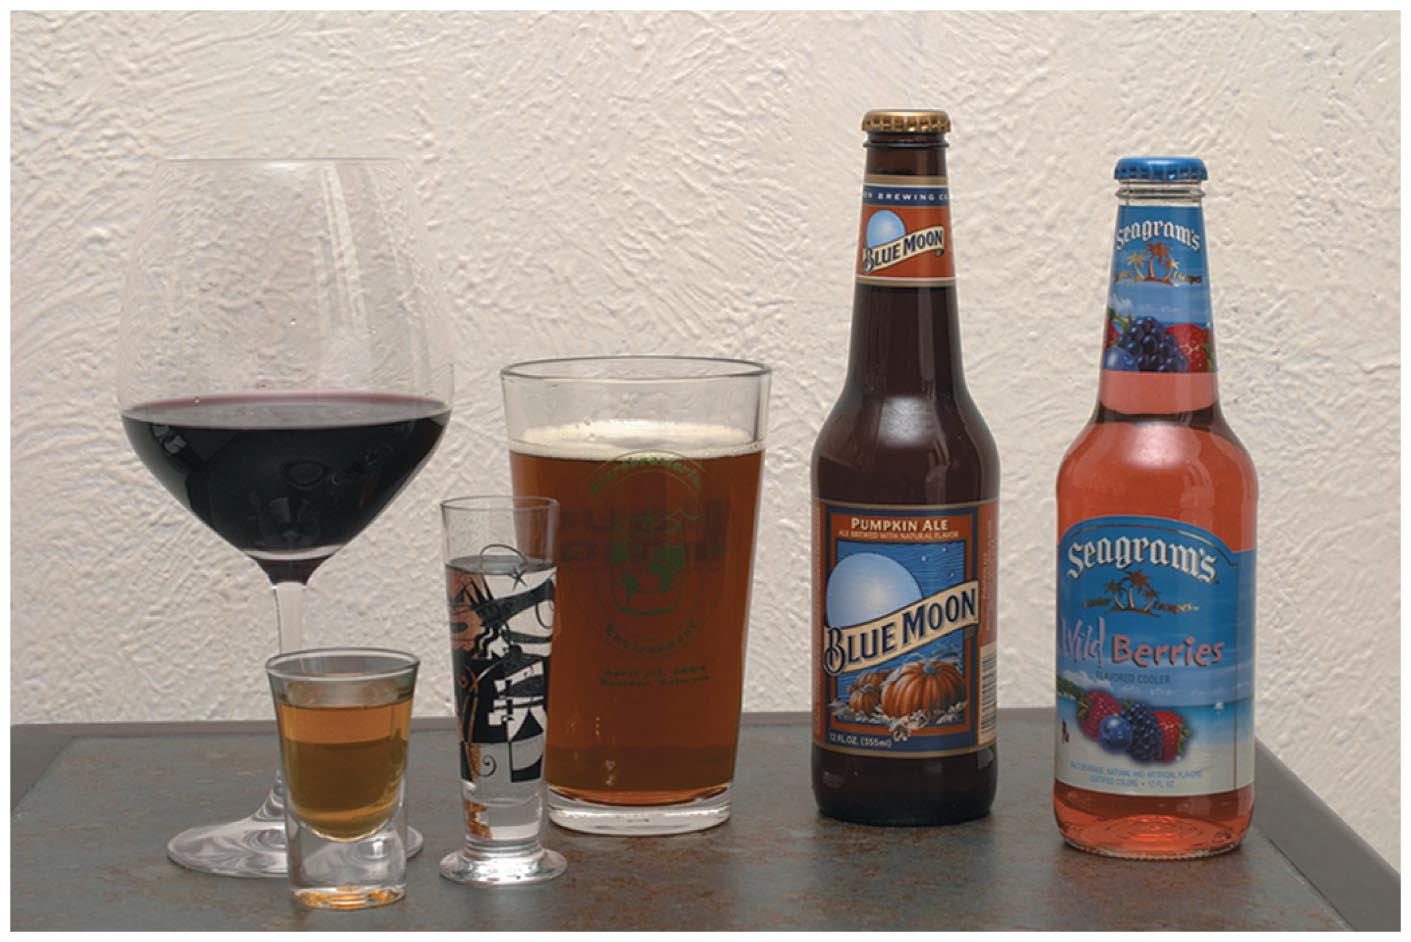
\includegraphics[width=\textwidth]{7_what_does_one_drink_look_like}
	\caption{What Does One Drink Look Like?}
	\label{fig:what_does_one_drink_look_like?}
\end{figure}

\begin{itemize}
	\item What is moderate alcohol intake?
	\begin{itemize}
		\item A \emph{drink} is defined as the amount of a beverage that provides $\frac{1}{2}$ fluid ounce of pure alcohol
		\item \definition{Proof}{a measurement of alcohol content}
		\item Moderate alcohol intake is defined as the consumption of up to one drink per day for women, and up to two drinks per day for men
	\end{itemize}
	\item Benefits of moderate consumption include
	\begin{itemize}
		\item Stress and anxiety reduction
		\item Appetite improvement
		\item Lower rates of heart disease
		\item Possible lower risks for diseases such as diabetes, heart disease, and liver disease
	\end{itemize}
	\item Concerns about moderate alcohol intake include
	\begin{itemize}
		\item Women appear to be at higher risk of breast cancer
		\item Increased risk of hypertension
		\item Higher rates of bleeding in the brain
		\item Relatively high Calorie content
		\item Potential risk of adverse drug interactions
	\end{itemize}
\end{itemize}

\begin{figure}[H]
	\centering
	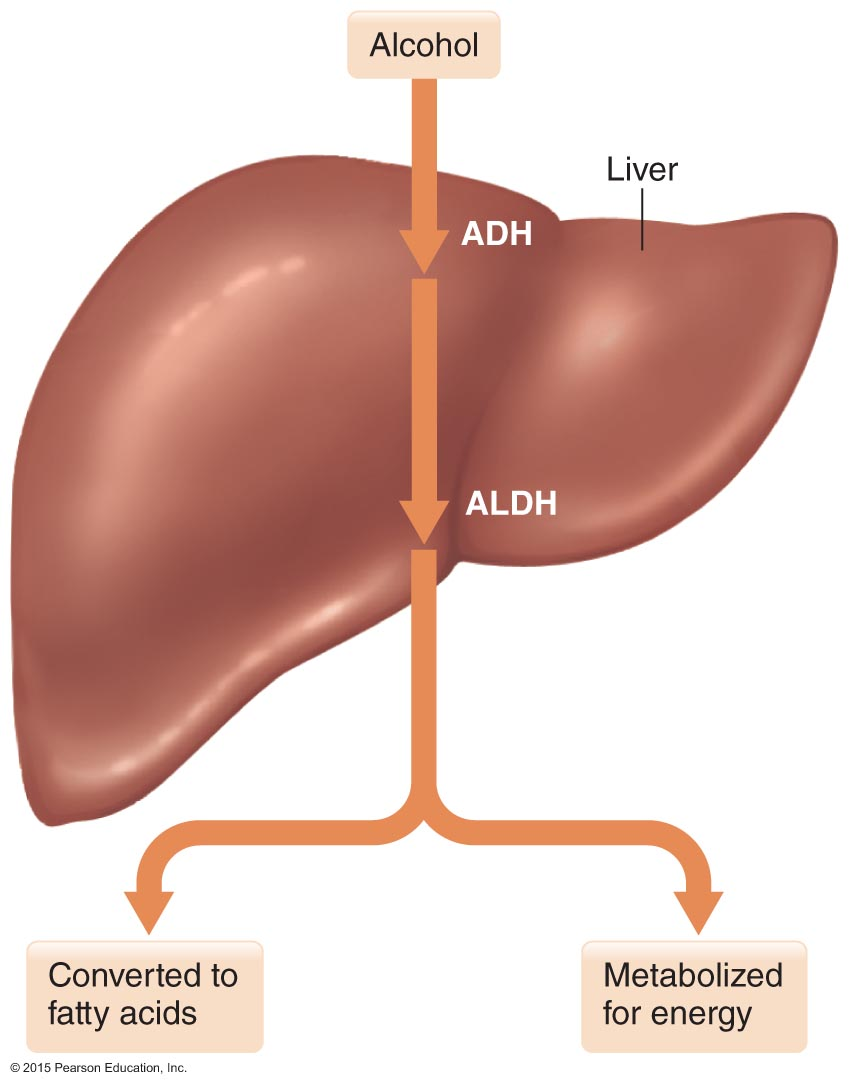
\includegraphics[width=0.5\textwidth]{7_metabolism_of_alcohol}
	\caption{Metabolism of Alcohol}
	\label{fig:metabolism_of_alcohol}
\end{figure}

\begin{table}[H]
	\centering
	\caption{Myths About Alcohol Metabolism}
	\label{tab:myths_about_alcohol_metabolism}
	\rowcolors{2}{rowmedgreen}{rowlightgreen}
	\begin{adjustbox}{max width=0.975\paperwidth,center}
		\begin{tabular}{p{0.5\paperwidth} p{0.5\paperwidth}}
			\rowcolor{rowdarkgreen}\textbf{The Claim} & \textbf{The Reality}\\
			Physical activity, such as walking around, will speed up the breakdown of alcohol. & Muscles don't metabolize alcohol; the liver does.\\
			Drinking a lot of coffee will keep you from getting drunk. & Coffee intake simply leaves you both wired and drunk.\\
			Using a sauna or steam room will force the alcohol out of your body. & Very little alcohol is lost in sweat; the alcohol will remain in your bloodstream.\\
			Herbal and nutritional products are available that speed up the breakdown of alcohol. & No commercial supplement is effective in increasing the rate of alcohol metabolism.\\
			\rowcolor{rowdarkgreen} & \\
		\end{tabular}
	\end{adjustbox}
\end{table}

\begin{itemize}
	\item Alcohol use disorder (AUD)
	\begin{itemize}
		\item Medical diagnosis for problem drinking that has become severe and is characterized by either abuse or dependence
	\end{itemize}
\end{itemize}

\subsection{Types Alcohol Abuse}\label{subsec:types-of-alcohol-abuse}
\subsubsection{Alcohol abuse}
excessive intake of alcohol
\subsubsection{Binge drinking}
consumption of five or more drinks per occasion
\subsubsection{Alcoholism}
a disease characterized by chronic dependence on alcohol

\subsection{Effects of alcohol abuse}\label{subsec:effects-of-alcohol-abuse}
\begin{itemize}
	\item A \emph{hangover} is a consequence of drinking too much alcohol; symptoms include headache, fatigue, dizziness, muscle aches and nausea
	\item Even at low intakes, alcohol impairs reasoning and judgement
	\item \definition{Alcohol poisoning}{a potentially fatal metabolic state involving cardiac or respiratory failure}
	\item Alcohol abuse can lead to traumatic injury from falls, drownings, assaults, and traffic accidents
\end{itemize}

\begin{figure}[H]
	\centering
	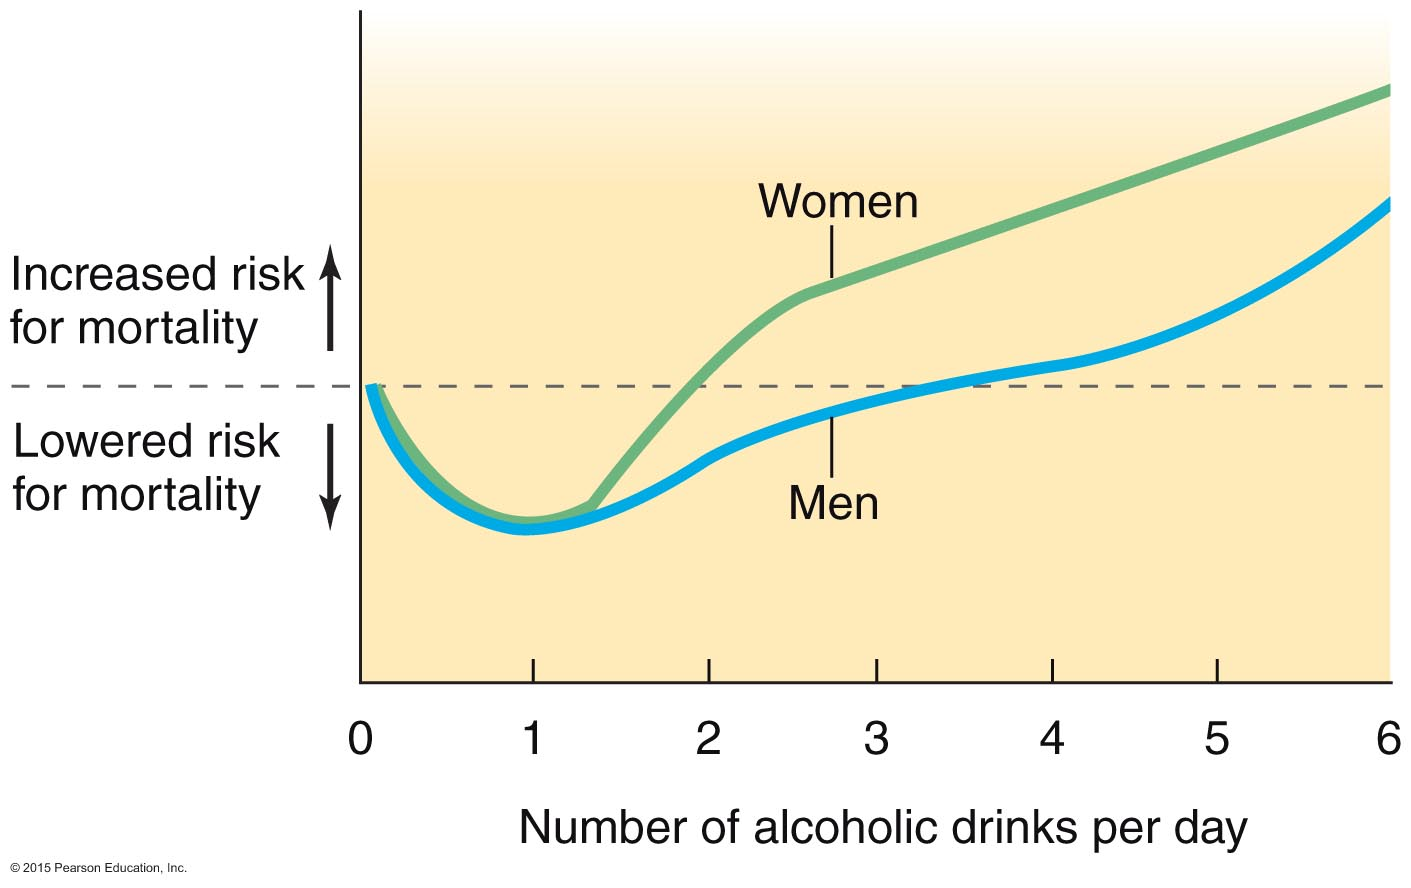
\includegraphics[width=\textwidth]{7_effects_of_alcohol_on_mortality_risk}
	\caption{Effects of Alcohol on Mortality Risk}
	\label{fig:effects_of_alcohol_on_mortality_risk}
\end{figure}

\begin{figure}[H]
	\centering
	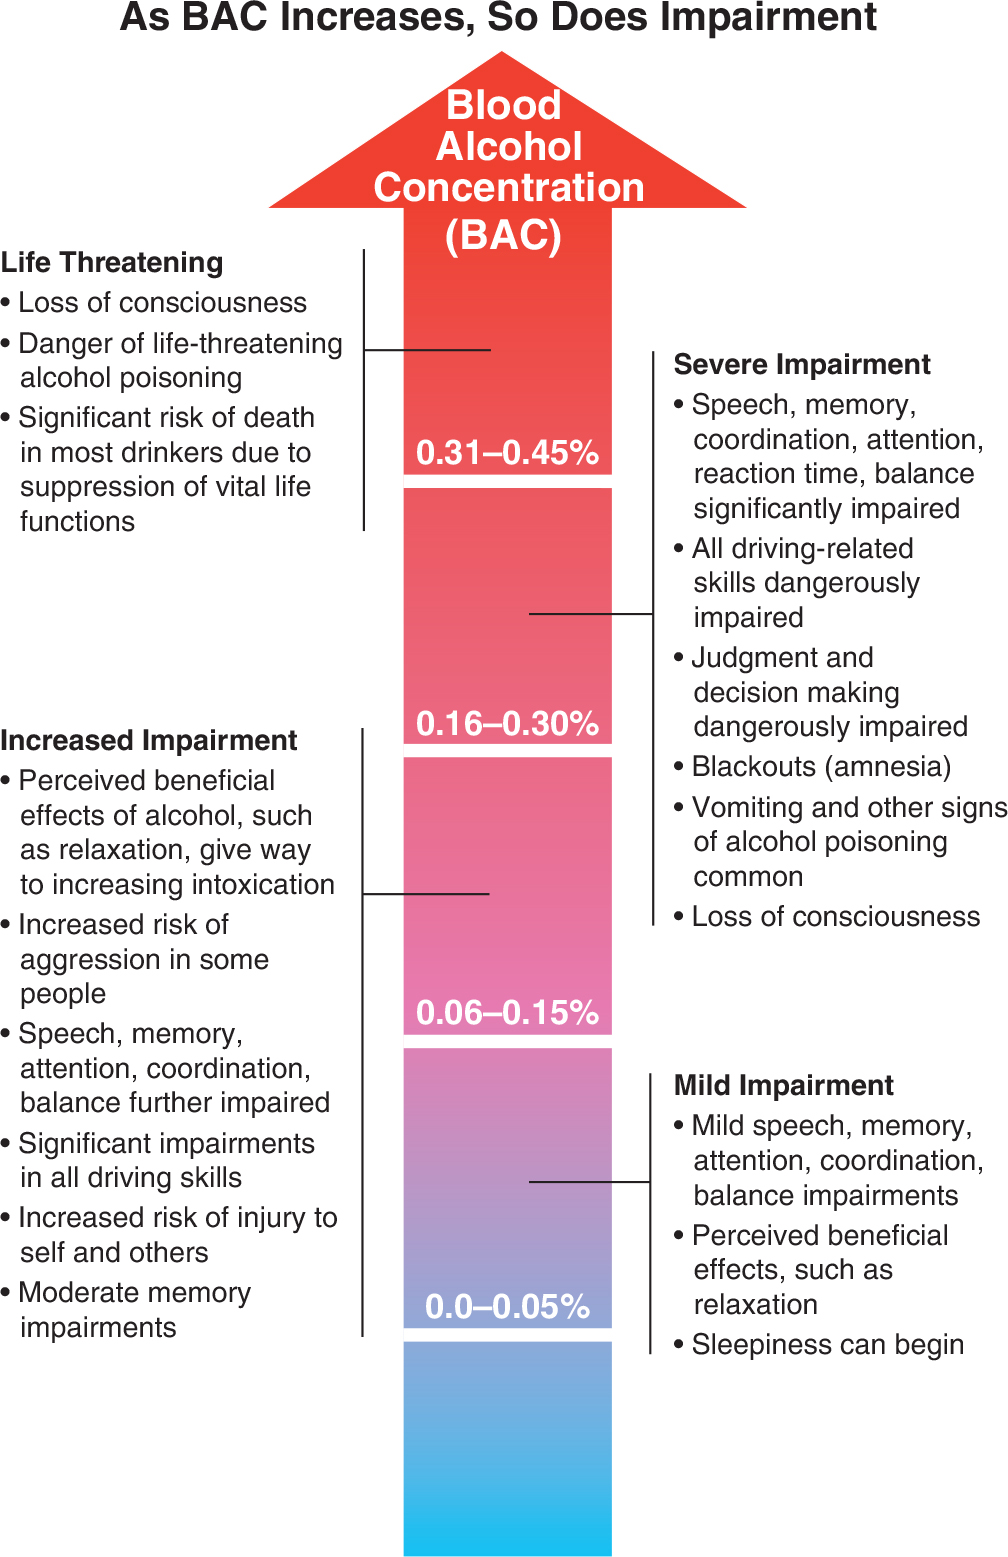
\includegraphics[height=0.5\paperheight]{7_effects_of_alcohol_on_brain_activity}
	\caption{Effects of Alcohol on Brain Activity}
	\label{fig:effects_of_alcohol_on_brain_activity}
\end{figure}

\begin{itemize}
	\item Effects of alcohol abuse:
	\begin{itemize}
		\item When the rate of alcohol intake exceeds the ability of the liver to break alcohol down, liver cells are damaged or destroyed
		\begin{description}
			\item[Fatty liver] is an early but reversible sign of liver damage
			\item[Alcohol hepatitis] results in loss of appetite, nausea and vomiting, abdominal pain, and jaundice
			\item[Cirrhosis of the liver] involves permanent scarring after years of alcohol abuse
		\end{description}
	\end{itemize}
\end{itemize}

\begin{figure}[H]
	\centering
	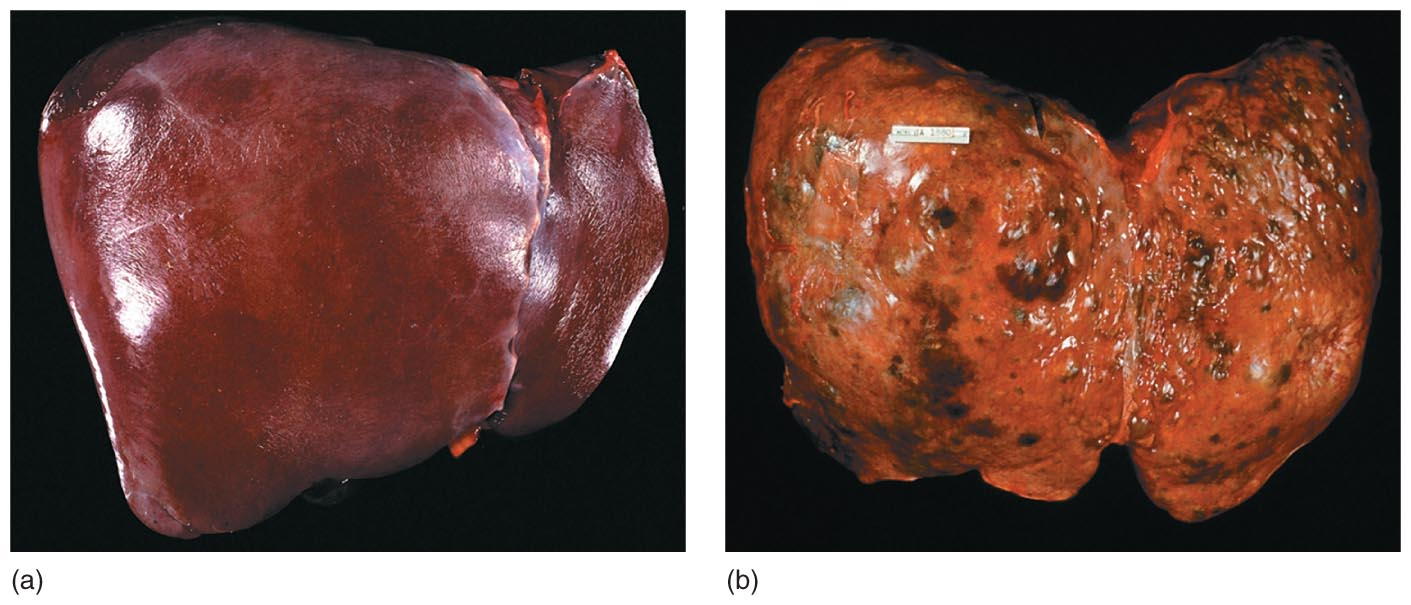
\includegraphics[width=\textwidth]{7_cirrhosis_of_the_liver}
	\caption{Cirrhosis of the liver}
	\label{fig:cirrhosis_of_the_liver}
\end{figure}

\begin{itemize}
	\item Chronically high intake increases risk of
	\begin{itemize}
		\item Impaired bone health
		\item Pancreatic injury and diabetes
		\item Cancer
		\item Abdominal obesity
		\item Malnutrition
	\end{itemize}
\end{itemize}

\begin{figure}[H]
	\centering
	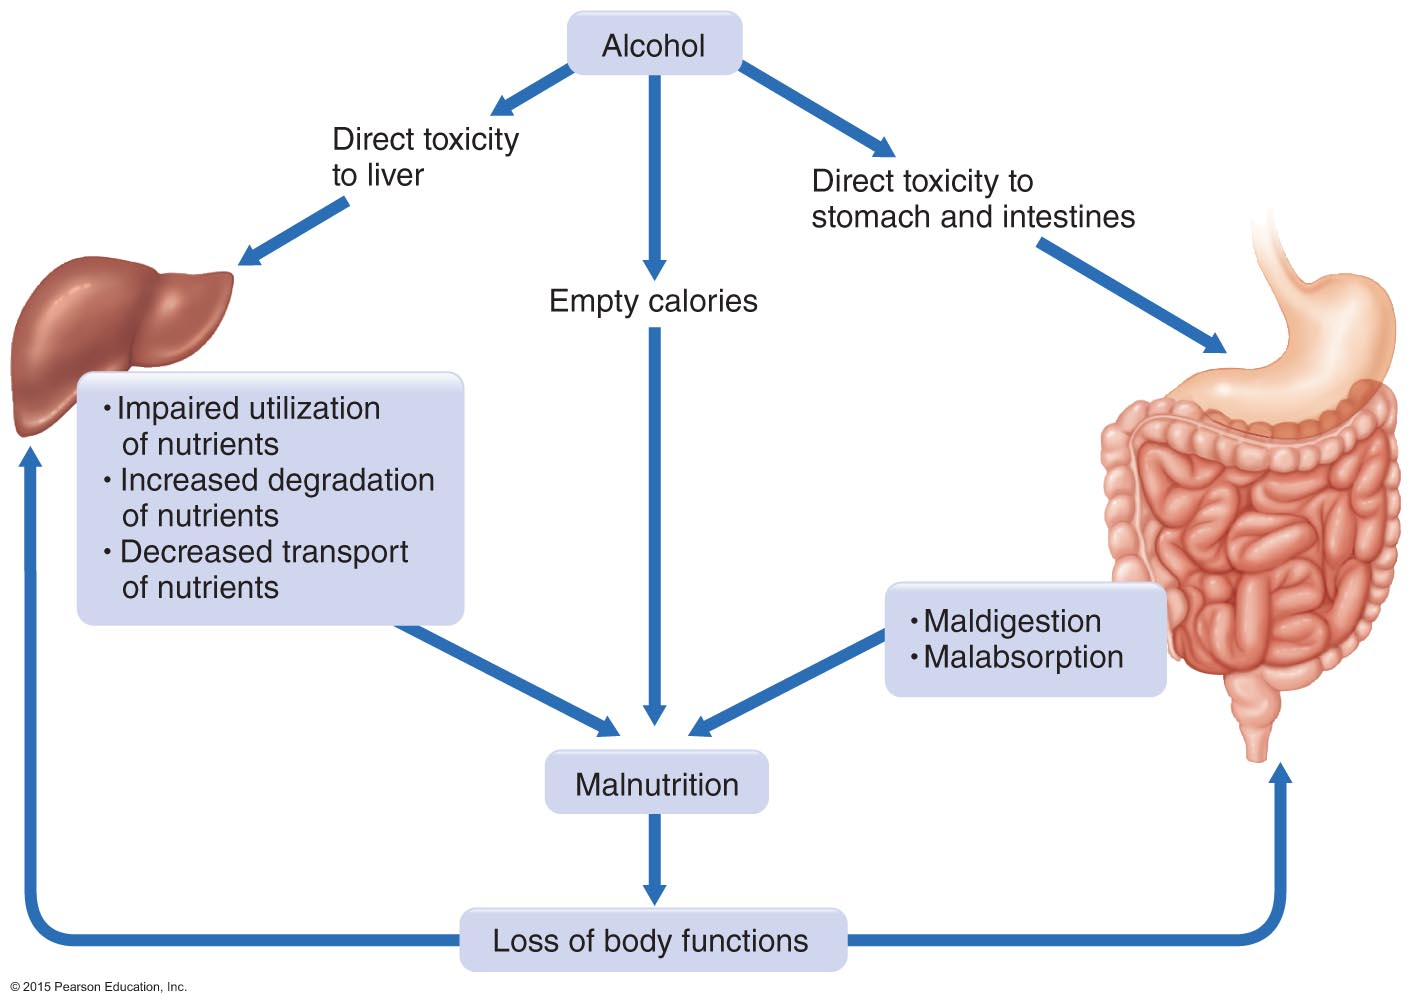
\includegraphics[width=\textwidth]{7_alcohol_related_malnutrition}
	\caption{Alcohol-Related Malnutrition}
	\label{fig:alcohol_related_malnutrition}
\end{figure}

\begin{itemize}
	\item Fetal and infant health problems include
	\begin{itemize}
		\item \definition{Fetal alcohol syndrome (FAS)\label{dfn:fas}}{a set of serious, irreversible birth defects, including physical, emotional, behavioral, and developmental problems}
		\item \definition{Fetal alcohol effects (FAE)\label{dfn:fae}}{subtler consequences that may be exhibited later, including hyperactivity, attention deficit disorder (ADD), and impaired learning abilities}
	\end{itemize}
\end{itemize}

\begin{figure}[H]
	\centering
	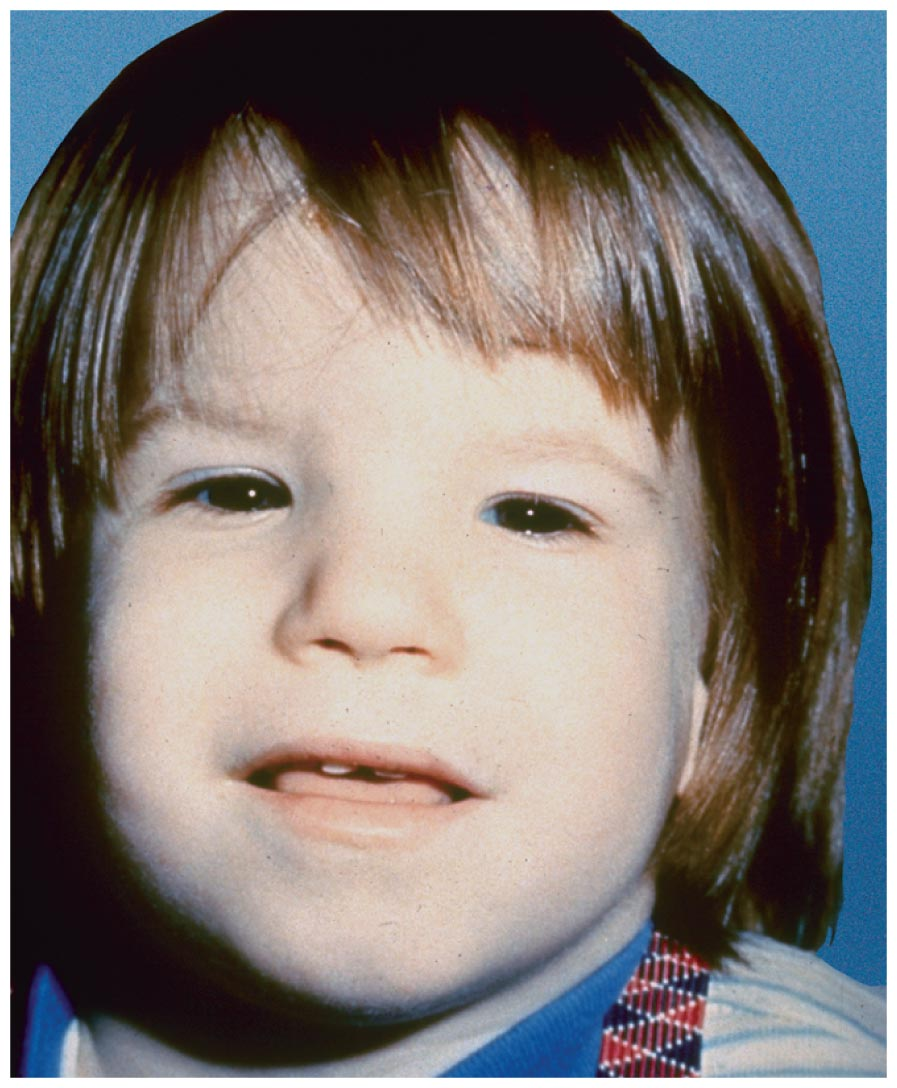
\includegraphics[width=\textwidth]{7_fetal_alcohol_syndrome}
	\caption{Fetal Alcohol Syndrome (FAS)}
	\label{fig:fetal_alcohol_syndrome}
\end{figure}

\begin{itemize}
	\item You should be concerned about your alcohol intake if you engage in binge drinking or drink at inappropriate times
	\item Speak with a trusted friend, coach, teacher, counselor, or healthcare provider
\end{itemize}

%</Chapter7>

\end{document}
